%------------------------------------------%
% Notes on Bayesian VAR
% Author: Keegan Skeate <keegan@cannlytics.com>
% Created: 2/25/2022
% Updated: 2/25/2022
%------------------------------------------%
\documentclass[11pt]{article}
\usepackage{titlesec}
\usepackage[top=.75in, bottom=.75in, left=0.75in, right=.75in]{geometry}
\usepackage[dvipsnames]{xcolor}
\usepackage{amssymb}
\usepackage{amsmath}
\usepackage{mathrsfs}
\usepackage{graphicx}
\usepackage{float}
\usepackage{booktabs}
\usepackage[singlelinecheck=off]{caption}
\usepackage{enumerate}
\usepackage{hhline}
\usepackage[justification=centering]{caption}

%------------------------------------------%
% Tables
%------------------------------------------%
\newcommand{\specialcell}[2][c]{%
  \begin{tabular}[#1]{@{}c@{}}#2\end{tabular}}
\newcommand\blfootnote[1]{\begingroup\renewcommand\thefootnote{}\footnote{#1}\addtocounter{footnote}{-1}\endgroup}
\usepackage{pbox}

%------------------------------------------%
% Format
%------------------------------------------%
\setlength{\parindent}{0pt}

%------------------------------------------%
% Document
%------------------------------------------%
\begin{document}

\noindent\Large {\bfseries\LARGE Notes on Bayesian Linear Regressions}\\Cannabis Data Science\\ Author: Keegan Skeate\\Written: \medskip\today

\vspace{\baselineskip}

$$
y_t = a_0 + \sum_{j=1}^p A_j y_{t-j} + \epsilon_t
$$

Common noninformative prior

$$
P(A, \Sigma)
$$

%------------------------------------------%
% Distributions
%------------------------------------------%
{\bfseries Pertinent Distributions} -- 

% Normal Distribution
\begin{minipage}{.45\textwidth}
\begin{figure}
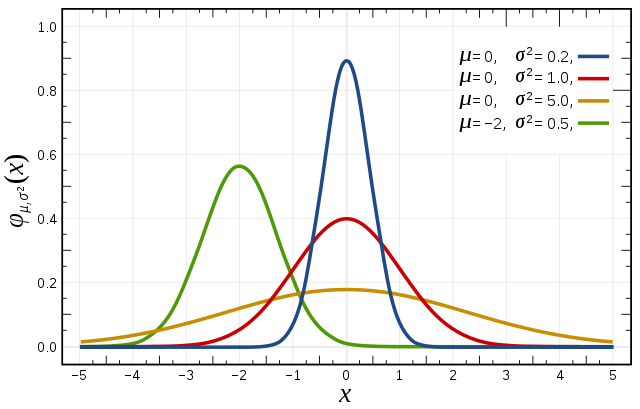
\includegraphics[height=1.1in]{images/normal-distribution.png}
\caption*{%
  \scriptsize
  {\bfseries Normal Distribution}\\[.5\baselineskip]
  Notation: $\mathcal{N}(\mu, \sigma^2)$\\[.5\baselineskip]
  Parameters: mean $\mu \in \mathbb{R}$, \\variance $\sigma^2 \in \mathbb{R}_{>0}$\\[.5\baselineskip]
  PDF:$p(x | \mu, \sigma^2) = \frac{1}{\sigma\sqrt{2\pi}}\text{exp}\left[ -\frac{1}{2}\left( \frac{x - \mu}{\sigma} \right)^2 \right]
$
}
\end{figure}
\end{minipage}\hspace{.05\textwidth}%
% Gamma Distribution
\begin{minipage}{.45\textwidth}
\begin{figure}
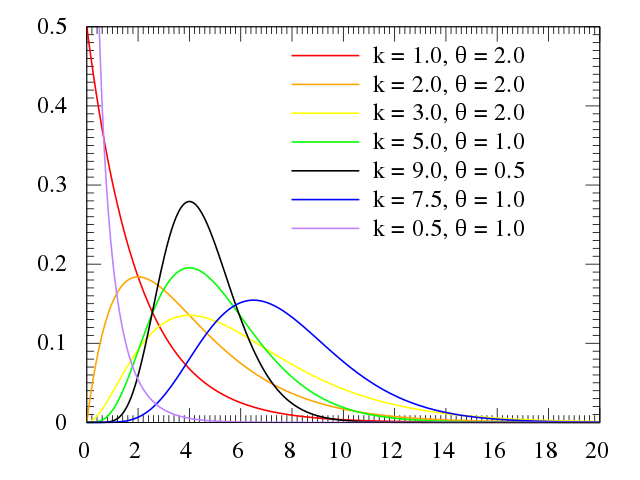
\includegraphics[height=1.1in]{images/gamma-distribution.png}
\caption*{%
  \scriptsize
  {\bfseries Gamma Distribution}\\[.5\baselineskip]
  Notation: $Y \sim G(\alpha, \beta)$\\[.5\baselineskip]
  Parameters: shape $\alpha > 0$, rate $\beta > 0$\\[.5\baselineskip]
  PDF:$
  f_\gamma(y | \alpha, \beta ) \equiv   \begin{cases}
    (\beta^\alpha \Gamma(\alpha))^{-1} y^{\alpha - 1}\text{exp}(-y /\beta)& \text{if } 0 < y < \infty \\
    0 & \text{otherwise.}
\end{cases}$
}
\end{figure}
\end{minipage}


% Inverse-gamma Distribution
\begin{minipage}{.3\textwidth}
\begin{figure}
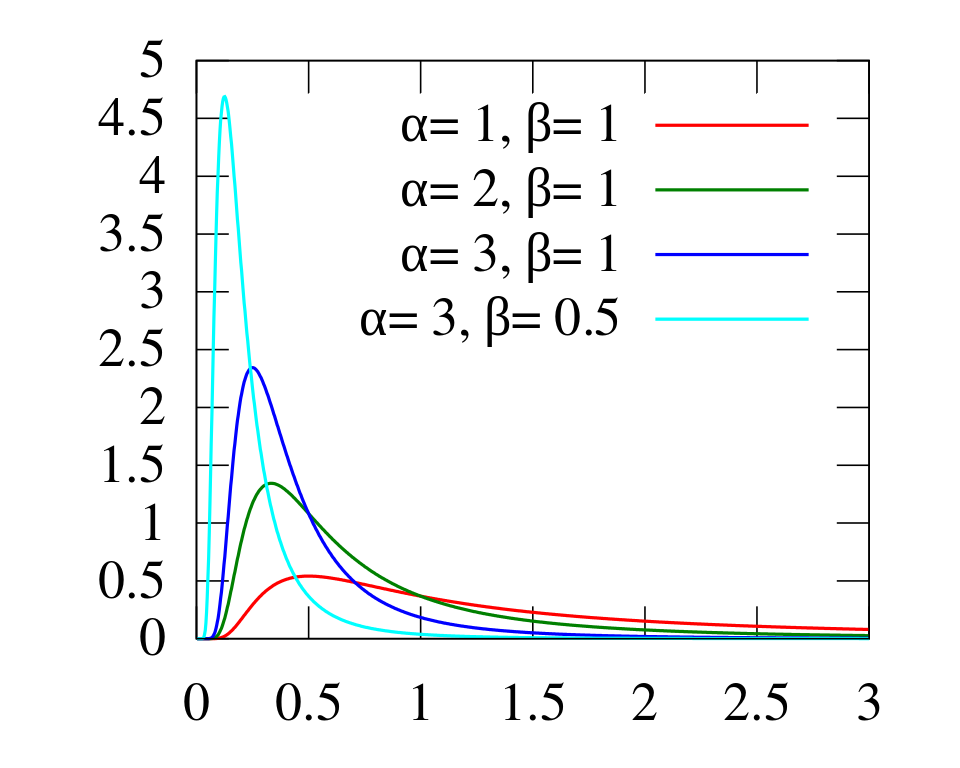
\includegraphics[height=\textwidth]{images/inverse-gamma-distribution.png}
\caption*{%
  \scriptsize
  {\bfseries Inverse-gamma Distribution}\\[.5\baselineskip]
  Notation: $Y \sim \mathcal{IG}(\alpha, \beta)$ \\[.5\baselineskip]
  Parameters: shape $\alpha > 0$, scale $\beta > 0$ \\[.5\baselineskip]
  PDF: $ p(y | \alpha, \beta) = [\Gamma(\alpha)\beta^\alpha]^{-1}y^{-(\alpha + 1)}\text{exp}(-1/[y\beta])$
}
\end{figure}
\end{minipage}\hspace{.15\textwidth}%
% Normal-inverse-gamma Distribution
\begin{minipage}{.55\textwidth}
\begin{figure}
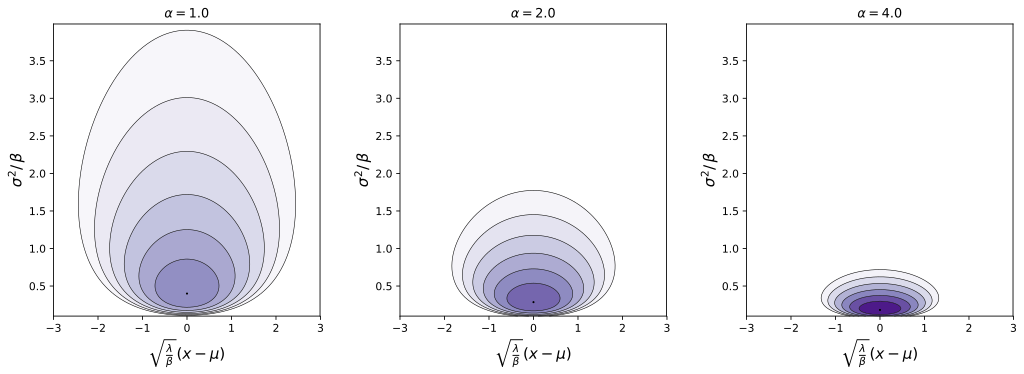
\includegraphics[width=\textwidth]{images/normal-inverse-gamma-distribution.png}
\caption*{%
  \scriptsize
  {\bfseries Normal-inverse-gamma Distribution}\\[.5\baselineskip]
  Notation: $(x, \sigma^2) \sim \mathcal{NIG}(\mu, \lambda, \alpha, \beta)$ \\[.5\baselineskip]
  Parameters: mean $\mu$, variance $\sigma^2/\lambda$, shape $\alpha > 0$, scale $\beta > 0$ \\[.5\baselineskip]
  PDF: $f(x, \sigma^2 | \mu, \lambda, \alpha, \beta) = \frac{\sqrt{\lambda}}{\sqrt{2\pi\sigma^2}}\frac{\beta^\alpha}{\Gamma(\alpha)}\left(\frac{1}{\sigma^2} \right)^{\alpha + 1}\text{exp}\left( -\frac{2\beta + \lambda(x - \mu)^2}{2\sigma^2} \right)$
 }
\end{figure}
\end{minipage}

\vfill
\begin{spacing}{0.5}
  {\tiny Credit: IkamusumeFan (Inverse-gamma distribution figure), Peter.komar.hu (Normal-inverse-gamma distribution figure)\\[.375\baselineskip]
  Licenses: https://creativecommons.org/licenses/by-sa/4.0/deed.en}
  {\tiny Gamma Distribution figure, \\ MarkSweep and Cburnett \\ License: https://creativecommons.org/licenses/by-sa/3.0/deed.en\\[-1\baselineskip] No changes were made to the figure.}
\end{spacing}



%------------------------------------------%
% Linear Regressions
%------------------------------------------%
\vspace{\baselineskip}
{\bfseries Linear Regressions} --


%------------------------------------------%
% The Classical Linear Regression
%------------------------------------------%
\vspace{\baselineskip}
{\bfseries The Classical Linear Regression} --


\vspace{\baselineskip}
{\bfseries The Bayesian Approach to Linear Regressions} --


% See pg.'s 142, 



In the posterior expression, $\beta$ enters only in the exponent

%$$
%
%$$

You can rewrite the exponent as

%$$
%
%$$

where


\vspace{\baselineskip}
\section*{References}

%Bayesian Econometric Methods ().


%------------------------------------------%
% Fin
%------------------------------------------%
\end{document}
